\chapter{Diseño de la plataforma}
\label{chap:diseno-plataforma}

\lettrine{E}{ste} capítulo define la organización del sistema propuesto y fija las decisiones de diseño que permiten operar con dos plataformas de adquisición distintas dentro de un mismo flujo de trabajo. El diseño se apoya en una idea simple: separar adquisición, comunicación, persistencia y operación para poder sustituir componentes sin romper el resto del sistema.

\section{Entorno y herramientas de desarrollo}

Antes de definir la arquitectura funcional, resulta conveniente fijar las herramientas de trabajo previstas para el desarrollo, las pruebas y la documentación técnica del sistema. Dado que el proyecto integra aplicación móvil, nodo embebido, scripts de análisis y documentación, no se utiliza una única herramienta de programación, sino un conjunto de entornos adaptados a cada parte del sistema.

El desarrollo general del repositorio se realiza con \textbf{Visual Studio Code}, que se emplea como editor principal para la memoria en LaTeX, los scripts de apoyo en Python, la revisión de ficheros de datos y la organización del código del proyecto. Esta herramienta resulta adecuada para mantener en un mismo espacio de trabajo la documentación, los experimentos y los componentes software auxiliares.

Para la aplicación Android se utiliza el entorno propio del ecosistema Android, basado en \textbf{Android Studio}, \textbf{Gradle} y el SDK de Android. Android Studio permite compilar, desplegar y depurar la aplicación en el dispositivo móvil, además de revisar el comportamiento de la interfaz y el acceso a sensores. Aunque parte del código pueda editarse desde Visual Studio Code, la validación práctica de la app se apoya en las herramientas oficiales de Android.

En la parte embebida se plantea una evolución por fases. En las primeras pruebas con el ESP32 y la IMU resulta útil emplear \textbf{Python/MicroPython} desde \textbf{Thonny}, ya que permite comprobar de forma rápida la conectividad, el bus I2C, la lectura básica del sensor y pequeños prototipos de comunicación sin cerrar todavía una implementación final. Una vez verificado el comportamiento básico del hardware, el desarrollo más fino del firmware se traslada a \textbf{C/C++}, usando el \textbf{IDE de Arduino} o una cadena equivalente de desarrollo para ESP32. Esta segunda fase permite mayor control sobre temporización, memoria, red, captura y generación de sesiones.

Para los scripts de análisis y pruebas de procesado se emplea \textbf{Python}, con librerías de cálculo y visualización para validar sesiones, comparar resultados y generar material de apoyo. Estos scripts no sustituyen al producto final, pero facilitan la exploración de parámetros, la depuración del pipeline y la preparación de resultados reproducibles para la memoria.

La capa de backend remoto queda como una línea de evolución. En esta fase no se fija todavía una tecnología definitiva, pero se consideran adecuadas alternativas de bajo coste y despliegue rápido como \textbf{Firebase} o \textbf{Supabase}, ya que ofrecen autenticación, base de datos, almacenamiento de ficheros y sincronización sin necesidad de mantener infraestructura propia. La elección final debe hacerse atendiendo a criterios de simplicidad, coste, trazabilidad de sesiones, facilidad de integración con Android y capacidad de evolucionar hacia escenarios con varios nodos.

Para los diagramas de diseño se utiliza una combinación de herramientas. Los primeros borradores se pueden definir con \textbf{Mermaid}, por su facilidad para versionar diagramas junto al código. Para las figuras finales de la memoria se pueden emplear herramientas gráficas como \textbf{diagrams.net} o figuras generadas específicamente para el documento, exportadas como imagen e integradas en LaTeX. En los casos donde convenga mantener el diagrama directamente dentro de la memoria, también puede utilizarse \textbf{TikZ}.

\section{Vista general del sistema}

La plataforma se organiza en cuatro bloques funcionales:

\begin{itemize}
  \item \textbf{adquisición}: captura de muestras y construcción de sesiones a partir de Android o ESP32;
  \item \textbf{comunicación}: intercambio de comandos de control y transferencia de datos entre nodos;
  \item \textbf{backend/persistencia}: almacenamiento local y posible sincronización remota;
  \item \textbf{interfaz/control}: operación del sistema, consulta de sesiones y visualización de resultados.
\end{itemize}

Sobre esta base, el sistema contempla dos modos operativos:

\begin{itemize}
  \item \textbf{modo móvil}: el propio dispositivo Android actúa como nodo de captura, almacenamiento y explotación local;
  \item \textbf{modo embebido}: el nodo ESP32 realiza la captura y Android actúa como consola de supervisión, control y descarga.
\end{itemize}

\begin{figure}[htbp]
  \centering
  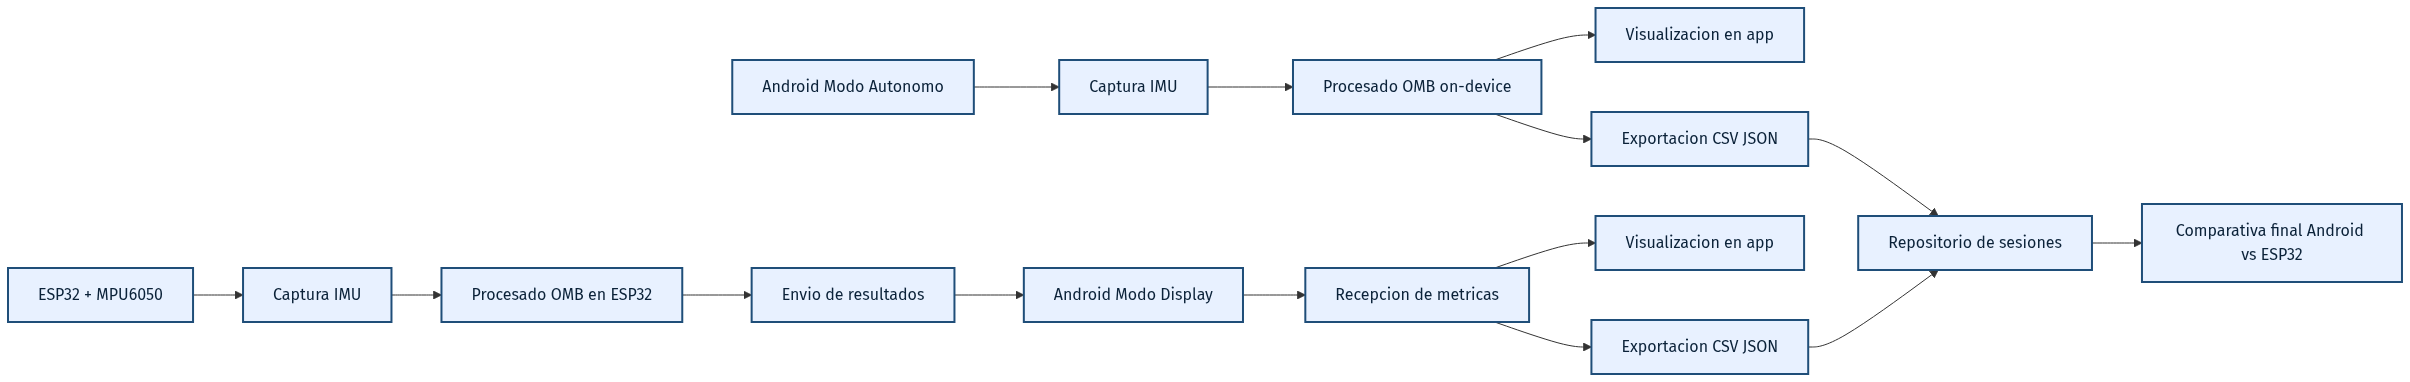
\includegraphics[width=0.98\textwidth]{imaxes/esquema_1_arquitectura.png}
  \caption{Arquitectura funcional del sistema con Android como plataforma central de operación.}
  \label{fig:plantilla-arquitectura}
\end{figure}

La decisión de mantener ambos modos dentro de un mismo diseño evita desarrollar dos soluciones independientes. El objetivo no es tener una aplicación móvil por un lado y un nodo embebido por otro, sino un único sistema capaz de operar con ambos.

\figplaceholder{%
Nombre propuesto: Diagrama de arquitectura general del sistema\\
Componentes recomendados: navegador/web, Android, ESP32, almacenamiento local y backend opcional
}{Hueco para diagrama de arquitectura general del sistema.}
\label{fig:placeholder-arquitectura-general}

\section{Diseño de adquisición}

La adquisición es el punto de entrada del sistema. Independientemente del origen de datos, toda captura debe poder convertirse en una sesión homogénea, de forma que el resto de la plataforma no dependa directamente del hardware que ha producido las muestras.

\subsection{Sesión como unidad de captura}

La sesión es la unidad principal de intercambio entre subsistemas. Toda captura, independientemente de su origen, debe quedar representada con una estructura común que permita almacenamiento, comparación y reprocesado.

El contrato de sesión incluye, como mínimo:

\begin{itemize}
  \item \texttt{device\_id};
  \item \texttt{source} (móvil/embebido/simulado);
  \item \texttt{timestamps};
  \item \texttt{fs} estimada;
  \item \texttt{payload} de muestras inerciales;
  \item metadatos de calidad y contexto.
\end{itemize}

Esta decisión permite que el procesado y la explotación trabajen con una entrada homogénea aunque el origen de datos cambie.

\subsection{Adquisición en Android}

En el modo móvil, el propio dispositivo Android actúa como nodo de captura. Registra las muestras del sensor, construye la sesión y permite una revisión inmediata del resultado desde la propia aplicación. Este modo constituye la base operativa del sistema porque reduce dependencia de hardware adicional y acelera la validación funcional.

La operación mínima en este modo incluye:

\begin{itemize}
  \item inicio y parada de captura;
  \item almacenamiento local de la sesión;
  \item consulta posterior y exportación.
\end{itemize}

\subsection{Adquisición en ESP32}

En el modo embebido, el nodo ESP32 se encarga de la captura y Android actúa como consola de operación. La sesión sigue siendo la misma unidad lógica de trabajo, aunque en este caso se genera fuera del teléfono y se recupera después a través de la capa de comunicación.

El subsistema embebido se compone de ESP32, IMU y electrónica auxiliar de conexión y alimentación. Su función es doble:

\begin{itemize}
  \item actuar como nodo de adquisición dedicado;
  \item servir como base de validación para la interoperabilidad con la app Android.
\end{itemize}

El diseño embebido debe garantizar, como mínimo:

\begin{itemize}
  \item captura de muestras y cierre de sesión;
  \item exposición de estado operativo;
  \item recepción de comandos de control;
  \item descarga posterior de la sesión generada.
\end{itemize}

\figplaceholder{%
Nombre propuesto: Diagrama de adquisición en doble modo\\
Comparativa recomendada: captura en Android frente a captura en ESP32 con sesión común
}{Hueco para diagrama de adquisición en modo móvil y modo embebido.}
\label{fig:placeholder-adquisicion-doble-modo}

\figplaceholder{%
Nombre propuesto: Esquema hardware del subsistema embebido\\
Contenido recomendado:\\
ESP32, IMU, conexiones relevantes y elementos de diagnóstico
}{Esquema del subsistema embebido y conexiones principales.}
\label{fig:placeholder-hardware-embebido}

\subsection{Separación entre captura y procesado}

El procesado se mantiene fuera de la capa de adquisición. Esta separación permite sustituir métodos de análisis sin alterar captura, comunicación o persistencia.

Cualquier bloque de procesado debe cumplir tres condiciones:

\begin{itemize}
  \item entrada basada en contrato de sesión;
  \item salida estructurada y trazable;
  \item compatibilidad con ambos orígenes de datos.
\end{itemize}

Sobre esa base, el sistema puede acomodar tanto métodos espectrales basados en PSD y momentos como otros enfoques apoyados en IMUs de baja precisión, transformación de aceleraciones al eje vertical, técnicas de denoising e integración en frecuencia.

\section{Diseño de comunicación}

La comunicación entre componentes debe permitir que la operación del sistema no quede ligada a una única plataforma de captura. En la práctica, esto implica que Android pueda actuar como nodo de sensado o como consola de control, manteniendo un flujo operativo comparable en ambos casos.

\subsection{Contrato de control}

Para la operación remota y la coordinación de nodos se define un contrato mínimo de control:

\begin{itemize}
  \item \texttt{start};
  \item \texttt{stop};
  \item \texttt{set\_config};
  \item \texttt{status}.
\end{itemize}

El contrato de control cubre lo estrictamente necesario para iniciar y detener capturas, consultar estado y modificar configuración sin acoplar el diseño a una implementación concreta de transporte.

\figplaceholder{%
Nombre propuesto: Diagrama de secuencia de operación remota\\
Actores recomendados: usuario, interfaz web, Android, ESP32
}{Hueco para diagrama de secuencia de operación remota.}
\label{fig:placeholder-secuencia-operacion-remota}

\subsection{Enlace entre Android y ESP32}

La capa de comunicación cubre dos escenarios distintos:

\begin{itemize}
  \item \textbf{enlace local Android-ESP32}, utilizado en laboratorio y en pruebas de integración;
  \item \textbf{sincronización remota con backend}, prevista para consulta y operación desacoplada.
\end{itemize}

El sistema se diseña para no depender desde el principio de una única tecnología de transporte. La interfaz entre nodos debe mantenerse estable aunque el mecanismo concreto evolucione.

Por este motivo, la elección final del mecanismo de comunicación entre Android y ESP32 no se fija únicamente por conveniencia de implementación. Debe apoyarse en una evaluación experimental de latencia, robustez, simplicidad de integración y comportamiento bajo concurrencia, de forma que la decisión técnica quede respaldada por medidas y no solo por preferencia de desarrollo.

\subsection{Flujo de datos del sistema}

El flujo de datos completo se define en cuatro pasos:

\begin{enumerate}
  \item adquisición de muestras;
  \item normalización y empaquetado de sesión;
  \item persistencia local y/o sincronización remota;
  \item recuperación para visualización, comparación y exportación.
\end{enumerate}

\figplaceholder{%
Nombre propuesto: Diagrama de flujo de datos del sistema\\
Pipeline recomendado:\\
sensor $\rightarrow$ sesión $\rightarrow$ persistencia $\rightarrow$ consulta $\rightarrow$ visualización
}{Flujo de datos extremo a extremo del sistema.}
\label{fig:placeholder-flujo-datos}

Este flujo es el mismo independientemente del origen de captura. La diferencia entre modo móvil y modo embebido no está en la explotación final, sino en quién produce la sesión y cómo se llega hasta ella.

\section{Diseño de persistencia y backend}

La persistencia se diseña con dos niveles complementarios:

\begin{itemize}
  \item \textbf{persistencia local}, necesaria para que cada nodo pueda cerrar sesiones de forma autónoma;
  \item \textbf{persistencia remota}, necesaria cuando se quiera sincronizar sesiones, estado de nodos o información de operación.
\end{itemize}

El backend se plantea como una capa intercambiable. Sus capacidades mínimas son:

\begin{itemize}
  \item persistencia de metadatos de sesión;
  \item almacenamiento de ficheros o exportaciones;
  \item sincronización de estado entre nodos.
\end{itemize}

La capa de explotación proporciona operaciones homogéneas de:

\begin{itemize}
  \item listado de sesiones;
  \item detalle de sesión;
  \item exportación de datos.
\end{itemize}

Este contrato permite que la app trate sesiones locales, embebidas o sincronizadas bajo el mismo flujo de trabajo. La selección tecnológica final de backend se deja abierta y se decidirá por criterios de validación práctica: robustez de despliegue, mantenibilidad, coste y capacidad de escalar hacia escenarios con más de un nodo.

\figplaceholder{%
Nombre propuesto: Diagrama de despliegue lógico y persistencia\\
Elementos recomendados: Android, almacenamiento local, ESP32, backend remoto opcional
}{Hueco para diagrama de despliegue lógico y persistencia.}
\label{fig:placeholder-despliegue-persistencia}

\section{Diseño de interfaz y control}

Android no se limita a la interfaz gráfica. Dentro del diseño propuesto, la aplicación asume tres funciones:

\begin{itemize}
  \item nodo de captura cuando se trabaja en modo móvil;
  \item consola de operación cuando se trabaja con el subsistema embebido;
  \item punto de acceso a sesiones, resultados y exportación.
\end{itemize}

En consecuencia, la interfaz debe soportar dos flujos principales: operación local sobre la propia captura del teléfono y operación remota sobre el nodo ESP32. En ambos casos, el objetivo es mantener una experiencia homogénea de inicio de captura, consulta de estado, recuperación de sesión y revisión de resultados.

\begin{figure}[htbp]
  \centering
  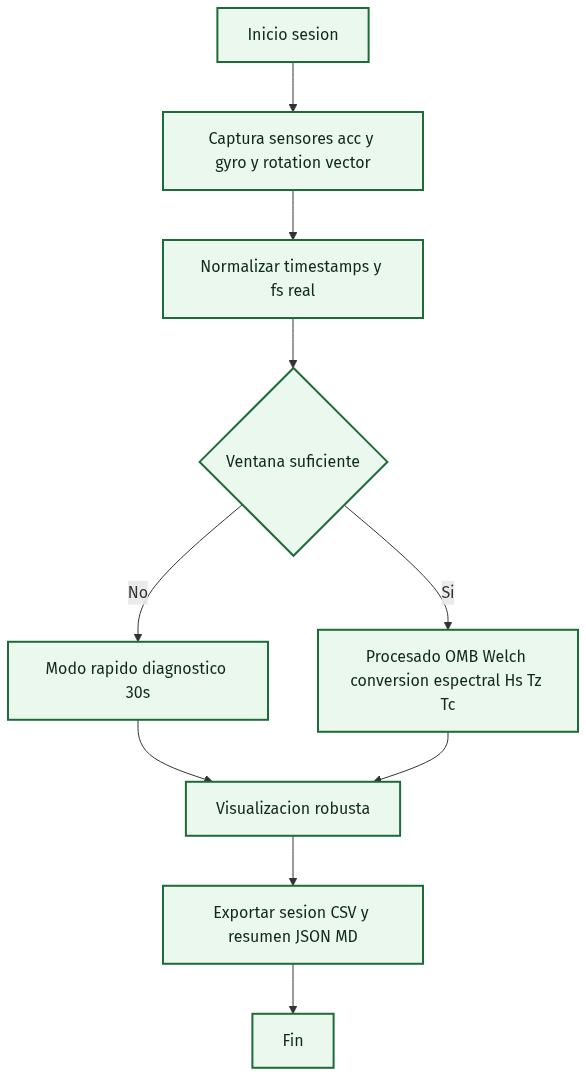
\includegraphics[width=0.65\textwidth]{imaxes/esquema_2_flujo_android.png}
  \caption{Flujo Android: captura/operación, gestión de sesiones y visualización.}
  \label{fig:plantilla-android}
\end{figure}

La comparativa entre plataformas forma parte de este diseño de interfaz y control. Para que la comparación tenga sentido, ambos modos deben compartir una estructura común de sesión, operaciones equivalentes de control y un flujo homogéneo de explotación.

\begin{figure}[htbp]
  \centering
  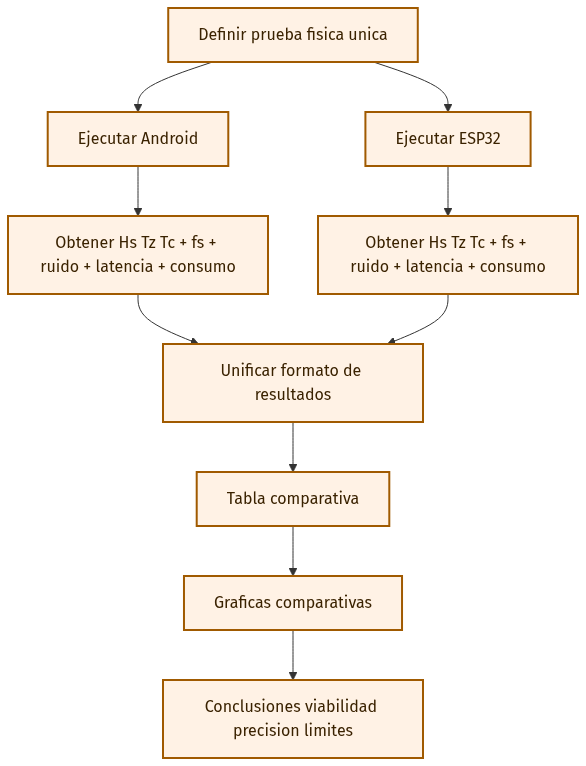
\includegraphics[width=0.62\textwidth]{imaxes/esquema_3_comparativa.png}
  \caption{Flujo de comparativa entre nodo móvil y nodo embebido con contratos comunes.}
  \label{fig:plantilla-comparativa}
\end{figure}

Los ejes principales de comparación son estabilidad de captura, trazabilidad de sesión, latencia operativa y robustez de integración. La intención no es comparar únicamente valores numéricos, sino también el coste operativo y el grado de control técnico que aporta cada plataforma.

\figplaceholder{%
Nombre propuesto: Diagrama de estados de operación\\
Estados recomendados: reposo, configurado, capturando, procesando, sesión disponible, error
}{Hueco para diagrama de estados de operación del sistema.}
\label{fig:placeholder-estados-operacion}
